%-------------------------------------------------------------------------
% corriges-ds-info-S1-instructions.tex
%-------------------------------------------------------------------------

%-------------------------------------------------------------------------
\documentclass[11pt,a4paper]{article}
%-------------------------------------------------------------------------

%-------------------------------------------------------------------------
\input{corriges-ds-info-S1-preambule.tex}
%-------------------------------------------------------------------------

%-------------------------------------------------------------------------
\begin{document}
%-------------------------------------------------------------------------

%-------------------------------------------------------------------------
\section{Affectation}
%-------------------------------------------------------------------------

\paragraph{Enoncé :} 
Un libraire propose une réduction de 3.5\% sur le prix hors taxes (HT) 
d'un livre à 12.35 \euro{} HT.
Sachant que la taxe sur la valeur ajoutée (TVA) sur les livres est de 5.5\%, 
proposer une instruction de type « affectation » qui permettra de calculer 
le prix final toutes taxes comprises (TTC) pour le client.
	
\paragraph{Méthode :}
On commence par s'abstraire 
des données spécifiques, en particulier numériques, pour ne considérer que les variables associées. 

Il s'agit ici de calculer le prix TTC (noté \texttt{ttc}) d'un produit
connaissant son prix HT (noté \texttt{ht}), la TVA (notée \texttt{tva} et
exprimée sous la forme d'un pourcentage) sur ce type de produit et 
la réduction éventuelle (notée \texttt{r} et exprimée sous la forme d'un 
pourcentage du prix HT) proposée par le vendeur sur ce produit.

Sachant qu'une réduction se soustrait du prix HT initial et 
qu'une taxe s'ajoute au prix hors taxes,
on a ainsi : \texttt{ttc = ht*(1-r/100)*(1+tva/100)} .

\paragraph{Résultat :}
Appliquer la méthode précédente revient simplement ici à initialiser les variables
\texttt{ht}, \texttt{r} et \texttt{tva} aux données du problème particulier.

\noindent\begin{minipage}{7cm}
Compte-tenu des valeurs de l'énoncé, le code \python{} ci-contre
permet de calculer le prix final TTC recherché.
\end{minipage}
\hfill
\begin{minipage}{8.25cm}
\begin{lstlisting}[caption=\textbf{prix d'un livre}]
ht, r, tva = 12.35, 3.5, 5.5
ttc = ht*(1-r/100)*(1+tva/100)
\end{lstlisting}
\end{minipage}

\paragraph{Vérification :} 
On peut utiliser une méthode d'encadrement du prix TTC
pour vérifier que la valeur obtenue est du bon ordre de grandeur.

Etant donné que \texttt{r < tva}, le prix TTC sera supérieur au prix HT et inférieur
au prix TTC sans réduction :
\texttt{ht < ttc < ht*(1+tva/100)}.

%-------------------------------------------------------------------------
\section{Tests}
%-------------------------------------------------------------------------

\paragraph{Enoncé :} 
Une grande surface propose un service de photocopies aux conditions suivantes :
les 100 premières pages sont facturées 0.1 \euro{} la page,
les 500 suivantes sont facturées 0.08 \euro{} la page
et au-delà, la page est facturée à 0.05 \euro{}.
Proposer une instruction de type «~alternative multiple~» 
qui permettra de calculer le prix total des photocopies pour un document 
de $n$ pages.

\paragraph{Méthode :}
On commence par s'abstraire 
des données spécifiques, en particulier numériques, pour ne considérer que les variables associées. 

Il s'agit ici de calculer le prix total \texttt{pt} de \texttt{nt} exemplaires
d'un produit sachant que le prix unitaire \texttt{p} du produit dépend du
nombre d'exemplaires selon le principe suivant.


\noindent\begin{minipage}{5cm}
Les \texttt{n1} premiers exemplaires sont facturés au prix unitaire \texttt{p1},
de \texttt{n1} à \texttt{n2} exemplaires le prix unitaire est \texttt{p2},
de \texttt{n2} à \texttt{n3} exemplaires le prix unitaire est \texttt{p3},
et ainsi de suite; 
au-delà de $n_m$ exemplaires le prix unitaire est \texttt{pm}.
\end{minipage}
\hfill
\begin{minipage}{10cm}
\begin{tikzpicture}[scale=1]\footnotesize\shorthandoff{:}
\draw (8,0) node[right] {$n$};
\draw (0,4.25) node[above] {$p(n)$};
\draw[->] (-0.25,0) -- (8,0);
\draw[->] (0,-0.25) -- (0,4.25);
\draw[fill] (0,0) circle(0.03);
\draw (1,0) node[below] {$n_1$};
\draw (3,0) node[below] {$n_2$};
\draw (6,0) node[below] {$n_3$};
\draw (0,4) node[left] {$p_1$};
\draw (0,3) node[left] {$p_2$};
\draw (0,2) node[left] {$p_3$};
\draw (0,1) node[left] {$p_m$};
\draw (0,4) -- (1,4);
\draw (1,3) -- (3,3);
\draw (3,2) -- (6,2);
\draw (6,1) -- (7,1);
\draw[dashed,->] (7,1) -- (8,1);
\draw[dashed] (1,0) -- (1,4);
\draw[dashed] (3,0) -- (3,3);
\draw[dashed] (6,0) -- (6,2);
\draw[dashed] (0,1) -- (6,1);
\draw[dashed] (0,2) -- (3,2);
\draw[dashed] (0,3) -- (1,3);
\draw (4,-0.5) node[below] {Nombre d'exemplaires};
\draw (-0.75,2) node[above,rotate=90] {Prix unitaire};
\end{tikzpicture}
\end{minipage}

Ainsi, si un client veut acheter \texttt{nt} exemplaires, l'alternative multiple suivante permet
de déterminer le prix total \texttt{pt} :

\begin{Verbatim}
if   nt < n1 : pt = nt*p1
elif nt < n2 : pt = n1*p1 + (nt-n1)*p2
elif nt < n3 : pt = n1*p1 + (n2-n1)*p2 + (nt-n2)*p3
...
else         : pt = n1*p1 + (n2-n1)*p2 + (n3-n2)*p3 + ... + (nt-nm)*pm
\end{Verbatim}

\paragraph{Résultat :}
Appliquer la méthode précédente revient simplement ici à identifier le nombre de plages
de prix concernées, ici 3 : \texttt{n1 = 100}, \texttt{n2 = 100+500 = 600} 
avec les prix unitaires \texttt{p1 = 0.1}, \texttt{p2 = 0.08} et
\texttt{pm = 0.05}.


\noindent\begin{minipage}{3.5cm}
Le code \python{} ci-contre
permet de calculer le prix total recherché
pour une valeur de \texttt{nt} donnée.
\end{minipage}
\hfill
\begin{minipage}{11.5cm}\footnotesize
\begin{lstlisting}[caption=\textbf{prix de photocopies}]
n1, n2 = 100, 600
p1, p2, pm = 0.1, 0.08, 0.05
if   nt < n1 : pt = nt*p1
elif nt < n2 : pt = n1*p1 + (nt-n1)*p2
else         : pt = n1*p1 + (n2-n1)*p2 + (nt-n2)*pm
\end{lstlisting}
\end{minipage}

\paragraph{Vérification :}
On peut ici tester certaines valeurs calculables « à la main » :\\
\texttt{nt = 1000 = 100+500+400} $\Rightarrow$ \texttt{pt = 100*0.1 + 500*0.08 + 400*0.05 = 10+40+20 = 70},\\
\texttt{nt = 500 = 100+400} $\Rightarrow$ \texttt{pt = 100*0.1 + 400*0.08 = 10+32 = 42}.

%-------------------------------------------------------------------------
\section{Boucles}
%-------------------------------------------------------------------------

\paragraph{Enoncé :}
Proposer une instruction de type « boucle » qui permettra de calculer l'intégrale $I = \int cos(x) dx$ 
sur l'intervalle $[-\frac{\pi}{4},\frac{\pi}{4}]$ par la méthode des rectangles.

\noindent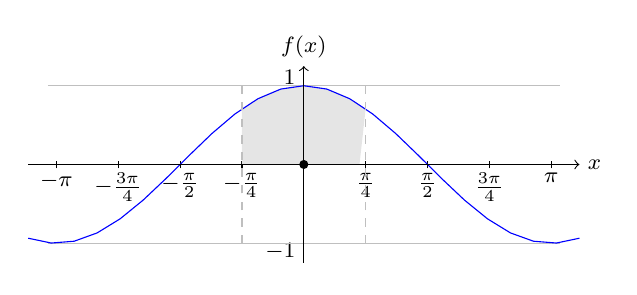
\begin{tikzpicture}[scale=1]\footnotesize\shorthandoff{:}
\draw (0,1.1) node[left] {$1$};
\draw (0,-1.1) node[left] {$-1$};
\draw[color=lightgray] (-3.25,1) -- (3.25,1) ;
\draw[color=lightgray] (-3.25,-1) -- (3.25,-1) ;
\draw ({-pi},-0.05) -- ({-pi},0.05);
\draw ({-pi},0) node[below] {$-\pi$};
\draw ({-3*pi/4},-0.05) -- ({-3*pi/4},0.05);
\draw ({-3*pi/4},0) node[below] {$-\frac{3\pi}{4}$};
\draw ({-pi/2},-0.05) -- ({-pi/2},0.05);
\draw ({-pi/2},0) node[below] {$-\frac{\pi}{2}$};
\draw ({-pi/4},-0.05) -- ({-pi/4},0.05);
\draw ({-pi/4},0) node[below] {$-\frac{\pi}{4}$};
\draw ({pi/4},-0.05) -- ({pi/4},0.05);
\draw ({pi/4},0) node[below] {$\frac{\pi}{4}$};
\draw ({pi/2},-0.05) -- ({pi/2},0.05);
\draw ({pi/2},0) node[below] {$\frac{\pi}{2}$};
\draw ({3*pi/4},-0.05) -- ({3*pi/4},0.05);
\draw ({3*pi/4},0) node[below] {$\frac{3\pi}{4}$};
\draw ({pi},-0.05) -- ({pi},0.05);
\draw ({pi},0) node[below] {$\pi$};
\draw[dashed,color=lightgray] ({-pi/4},-1) -- ({-pi/4},1);
\draw[dashed,color=lightgray] ({pi/4},-1) -- ({pi/4},1);
\fill[color=gray!20] ({-pi/4},0) -- ({-pi/4},{cos((-pi/4) r)}) -- plot [domain=(-pi/4):(pi/4)] (\x,{cos(\x r)}) -- ({cos((pi/4) r)},0) -- cycle;
\draw[color=blue,domain=-3.5:3.5] plot (\x,{cos(\x r)});
\draw[dashed,color=lightgray] ({-pi/4},-1) -- ({-pi/4},1);
\draw[dashed,color=lightgray] ({pi/4},-1) -- ({pi/4},1);
\draw[->] (0,-1.25) -- (0,1.25) ;
\draw (0,1.25) node[above] {$f(x)$};
\draw[->] (-3.5,0) -- (3.5,0) ;
\draw (3.5,0) node[right] {$x$};
\draw[fill] (0,0) circle (0.05);
\end{tikzpicture}
\hfill
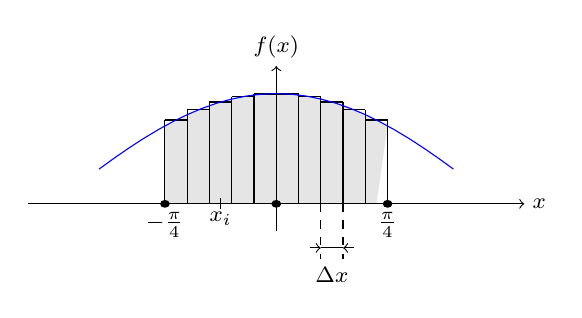
\begin{tikzpicture}[xscale=1.8,yscale=1.4]\footnotesize\shorthandoff{:}
\fill[color=gray!20] ({-pi/4},0) -- ({-pi/4},{cos((-pi/4) r)}) -- plot [domain=(-pi/4):(pi/4)] (\x,{cos(\x r)}) -- ({cos((pi/4) r)},0) -- cycle;
\foreach \x in {0,1,...,4} \draw ({-pi/4 + \x*pi/20},0) -- ({-pi/4 + \x*pi/20},{cos((-pi/4 + (\x+0.5)*pi/20) r)});
\foreach \x in {0,1,...,4} \draw ({-pi/4 + \x*pi/20},{cos((-pi/4 + (\x+0.5)*pi/20) r)}) -- ({-pi/4 + (\x+1)*pi/20},{cos((-pi/4 + (\x+0.5)*pi/20) r)});
\foreach \x in {0,1,...,4} \draw ({pi/4 - \x*pi/20},0) -- ({pi/4 - \x*pi/20},{cos((pi/4 - (\x+0.5)*pi/20) r)});
\foreach \x in {0,1,...,4} \draw ({pi/4 - \x*pi/20},{cos((pi/4 - (\x+0.5)*pi/20) r)}) -- ({pi/4 - (\x+1)*pi/20},{cos((pi/4 - (\x+0.5)*pi/20) r)});
\draw[color=blue,domain=-1.25:1.25] plot (\x,{cos(\x r)});
\draw[->] (0,-0.25) -- (0,1.25) ;
\draw[->] (-1.75,0) -- (1.75,0) ;
\draw (1.75,0) node[right] {$x$};
\draw (0,1.25) node[above] {$f(x)$};
\draw ({-pi/4},0) node[below] {$-\frac{\pi}{4}$};
\draw ({pi/4},0) node[below] {$\frac{\pi}{4}$};
\draw ({-pi/4 + 2.5*pi/20},0) node[below] {$x_i$};
\draw ({-pi/4 + 2.5*pi/20},-0.05) -- ({-pi/4 + 2.5*pi/20},0.05);
\draw ({2.5*pi/20},-0.5) node[below] {$\Delta x$};
\draw[dashed] ({2*pi/20},0) -- ({2*pi/20},-0.5);
\draw[dashed] ({3*pi/20},0) -- ({3*pi/20},-0.5);
\draw[->] ({1.5*pi/20},-0.4) -- ({2*pi/20},-0.4);
\draw[->] ({3.5*pi/20},-0.4) -- ({3*pi/20},-0.4);
\draw ({3*pi/20},-0.4) -- ({2*pi/20},-0.4);
\draw[fill] (0,0) circle(0.03);
\draw[fill] ({-pi/4},0) circle(0.03);
\draw[fill] ({pi/4},0) circle(0.03);
\end{tikzpicture}

\paragraph{Méthode :}
Il s'agit ici d'intégrer une fonction continue $f$ de $\mathbb{R} \rightarrow \mathbb{R}$ 
sur un intervalle $[a,b]$.
On supposera que $f$ à toutes les bonnes propriétés mathématiques pour être
intégrable sur l'intervalle considéré. 

On cherche donc à calculer l'intégrale
$\displaystyle I = \int_a^b f(x)dx$ qui représente classiquement l'aire
comprise entre la courbe représentative de $f$ et les droites d'équations 
$x=a$, $x=b$ et $y=0$. Les méthodes d'intégration numérique consistent 
essentiellement à trouver une bonne approximation de cette aire.

Dans la méthode des rectangles proposée, on subdivise l'intervalle d'intégration de
longueur $b-a$ en $n$ parties égales de longueur $\displaystyle\Delta x = \frac{b-a}{n}$. 
Soient $x_1$, $x_2$, \ldots, $x_n$ les points milieux de ces $n$ intervalles. 
Les $n$ rectangles formés avec les ordonnées correspondantes ont pour surface 
$f(x_1)\Delta x$, $f(x_2)\Delta x$, \ldots, $f(x_n)\Delta x$. 
L'aire sous la courbe est alors assimilée à la somme des aires de ces rectangles, soit 
$$\displaystyle I = \int_a^b f(x)dx \approx \left(f(x_1)+f(x_2)+\cdots+f(x_n)\right)\Delta x = 
\Delta x\cdot\sum_{i=1}^{i=n}f(x_i)$$ 
C'est la formule dite des rectangles qui repose sur une approximation par une fonction 
{\em en	escalier}.

Le calcul attendu revient donc à évaluer d'abord la somme $s = \sum f(x_i)$ puis
à la multiplier par la largeur $w = \Delta x$ des petits rectangles. 
Pour calculer $s$ « de tête »,
on évalue d'abord $f(x_1)$ que l'on mémorise : $s = f(x_1)$, 
puis on rajoute $f(x_2)$ et on mémorise cette somme intermédiaire : 
$s = s + f(x_2) \ (= f(x_1) + f(x_2))$, 
puis on rajoute $f(x_3)$ et on mémorise cette nouvelle somme intermédiaire  
$s = s + f(x_3) \ (= f(x_1) + f(x_2) + f(x_3))$
et ainsi de suite jusqu'à rajouter enfin $f(x_n)$ : 
$s = s + f(x_n) \ (= f(x_1) + f(x_2) + f(x_3) + \ldots + f(x_n))$. 
On a alors la somme recherchée ($s = \sum f(x_i)$) et
il ne reste plus qu'à multiplier cette somme $s$ par la largeur $w$ pour obtenir la valeur de l'intégrale $I$.

Les 4 étapes de construction de la boucle recherchée sont donc les suivantes :
\begin{itemize}
\item pour l'invariant, on vérifie qu'à chaque étape $k$, $s_k$ est toujours égal à la somme 
	des $k$ premiers termes $f(x_k)$ : 
	$\displaystyle \forall k, s_k = \sum_{i=1}^k f(x_i)$;
\item l'initialisation consiste à définir $w$, à se positionner sur le premier rectangle 
	$x_1 = a + w/2$ et à initialiser $s_1$ en conséquence : $s_1 = f(x_1)$;
\item la progression consiste à se déplacer sur le rectangle suivant : $x_{k+1} = x_{k} + w$
	et à augmenter $s_k$ de la nouvelle valeur $f(x_{k+1})$ afin de conserver l'invariant :
	$s_{k+1} = s_k + f(x_{k+1})$;
\item la condition d'arrêt est obtenue pour $x_k > b - w/2$.
\end{itemize}
\vspace*{3mm}

\noindent La boucle prend ainsi la forme :\\
\begin{minipage}[t]{8cm}
\begin{Verbatim}
« initialisation »
while not « condition d'arrêt » :
    « progression »
\end{Verbatim}
\end{minipage}
\hfill
\begin{minipage}[t]{7cm}\footnotesize
$w = (b-a)/2$, $x = x_1 = a + w/2$, $s = f(x_1)$\\
\texttt{while not} $x > b-w/2$ \texttt{:}\\
\mbox{}\texttt{\ \ \ \ } $x = x_{k+1} = x_{k} + w$\\
\mbox{}\texttt{\ \ \ \ } $s = s_{k+1} = s_k + f(x_{k+1})$\\
\end{minipage}

\paragraph{Résultat:} On applique la méthode précédente à la fonction $f : x \mapsto \cos(x)$
dans l'intervalle $\displaystyle \left[a=-\frac{\pi}{4},b=\frac{\pi}{4}\right]$.

\noindent\begin{minipage}{7cm}
Le code \python{} ci-contre permet de calculer l'intégrale recherchée
à condition de ne pas oublier de définir $f$, $a$, $b$ et $n$
avant d'exécuter la boucle précédente. On prendra par exemple $n = 100$.
\end{minipage}
\hfill
\begin{minipage}{8cm}\footnotesize
\begin{lstlisting}[caption=\textbf{intégration numérique}]
from math import *
f, a, b = cos, -pi/4, pi/4
n = 100
w = (b - a)/n
x = a + w/2
s = f(x)
while not (x > (b - w/2)):
    x = x + w
    s = s + f(x)
s = w*s
\end{lstlisting}
\end{minipage}

\paragraph{Vérification :}
On sait calculer analytiquement l'intégrale demandée :
$$I = \int_{-\frac{\pi}{4}}^{\frac{\pi}{4}} \cos(x) dx = \left[\sin(x)\rule[-0.25cm]{0cm}{0.5cm}\right]_{-\frac{\pi}{4}}^{\frac{\pi}{4}} = sin(\frac{\pi}{4}) - sin(-\frac{\pi}{4}) = \frac{\sqrt{2}}{2} - (-\frac{\sqrt{2}}{2}) =  2\frac{\sqrt{2}}{2} = \sqrt{2}$$
Ainsi, doit-on trouver une valeur proche de $\sqrt{2} \approx 1.414$.

%-------------------------------------------------------------------------
\section{Instructions imbriquées}
%-------------------------------------------------------------------------

\paragraph{Enoncé :}
Ecrire un algorithme qui permettra de déterminer le zéro de $\cos(x)$ dans $[1,2]$ selon une méthode
par dichotomie.

\begin{minipage}{6cm}
\begin{tikzpicture}[xscale=1.4,yscale=1.4]\footnotesize\shorthandoff{:}
\draw[color=blue,domain=0.25:2.75] plot (\x,{cos(\x r)});
\draw[dashed] (1,-1) -- (1,1);
\draw[dashed] (2,-1) -- (2,1);
\draw[dashed] (-0.25,-1) -- (3.25,-1);
\draw[dashed] (-0.25,1) -- (3.25,1);
\draw[fill] (0,0) circle(0.03);
\draw[fill] (1,0) circle(0.03);
\draw[fill] (2,0) circle(0.03);
\draw[fill] (3,0) circle(0.03);
\draw (0,-0.15) node[left] {0};
\draw (1,-0.15) node[left] {1};
\draw (2,-0.15) node[left] {2};
\draw (3,-0.15) node[left] {3};
\draw[->] (0,-1.25) -- (0,1.25) ;
\draw[->] (-0.25,0) -- (3.25,0) ;
\draw (3.25,0) node[right] {$x$};
\draw (0,1.25) node[above] {$f(x)$};
\end{tikzpicture}
\end{minipage}
\hfill
\begin{minipage}{8cm}
Indications : Soient $[x_1,x_2]$ l'intervalle de recherche et $x_m = (x_1+x_2)/2$ le point milieu 
de cet intervalle. Si $f(x_1)\cdot f(x_m) < 0$, le zéro recherché est dans $[x_1,x_m]$, sinon le
zéro est dans $[x_m,x_2]$. On réitère le procédé sur le nouvel intervalle de recherche jusqu'à ce que
la longueur de l'intervalle soit suffisamment petite. Le milieu de ce dernier intervalle sera le
zéro recherché.
\end{minipage}

\paragraph{Méthode :}
\begin{tikzpicture}[xscale=4]\footnotesize\shorthandoff{:}
\draw[color=blue,domain=1:3] plot (\x,{cos(\x r)});
\draw[dashed,color=lightgray] (1,-1.25) -- (1,1.25);
\draw (1,-0.25) node[left] {$a$};
\draw[dashed,color=lightgray] (3,-1.25) -- (3,1.25);
\draw (3,-0.25) node[right] {$b$};
\draw (2,0) node[above] {$x_1$};
\draw (2,-0.05) -- (2,0.05);
\draw (1.5,0) node[above] {$x_2$};
\draw (1.5,-0.05) -- (1.5,0.05);
\draw (1.75,0) node[above] {$x_3$};
\draw (1.75,-0.05) -- (1.75,0.05);
\draw (1.625,0) node[above] {$x_4$};
\draw (1.625,-0.05) -- (1.625,0.05);
\draw (1.5625,0) node[below] {$x_5$};
\draw (1.5625,-0.05) -- (1.5625,0.05);
\draw[->] (0.9,0) -- (3.1,0) ;
\draw (3.1,0) node[right] {$x$};
\end{tikzpicture}

\paragraph{Résultat :}\mbox{}

\noindent\begin{minipage}{7cm}
Le code \python{} ci-contre permet de calculer le zéro de la fonction cosinus
dans l'intervalle $[1,2]$.
Pour le seuil de précision, on prendra par exemple
$s = 10^{-9}$.
\end{minipage}
\hfill
\begin{minipage}{8cm}\footnotesize
\begin{lstlisting}[caption=\textbf{zéro d'une fonction}]
from math import *
f, a, b = cos, 1, 2
s = 1.e-9
x1, x2 = a, b
x = (x1 + x2)/2
while not ((x2 - x1) <= s):
    if f(x1)*f(x) < 0 : x2 = x
    else              : x1 = x
    x = (x1 + x2)/2
\end{lstlisting}
\end{minipage}
    
\paragraph{Vérification :}
On connaît les zéros de la fonction cosinus : ce sont
tous les multiples de $\pi/2$;
ainsi, dans l'intervalle $[1,2]$ doit-on trouver une valeur proche de
$\pi/2 \approx 1.57$.


%-------------------------------------------------------------------------
\section{Exécution d'une séquence d'instructions}
%-------------------------------------------------------------------------

\paragraph{Enoncé :}
On considère la séquence d'instructions suivantes :

\begin{lstlisting}
n = 0
while n <= k:
    j = 0
    while j <= n:
        num, den = 1, 1
        i = 1
        while i <= j:
            num = num * (n - i + 1)
            den = den * i
            i = i + 1
        c = num//den
        print(c,end=' ')
        j = j + 1
    print()
    n = n + 1
\end{lstlisting}
\vspace*{3mm}

\noindent Qu'affiche cette séquence pour \texttt{k = 6} ?

\paragraph{Réponse :} On n'attend pas ici une réponse concernant la méthode (M).
En guise de vérification (V), on pourra proposer un nom à cet algorithme.

\paragraph{Méthode :}
Pour suivre « à la main » l'exécution d'une série de boucles imbriquées, 
on calcule les valeurs de toutes les variables impliquées à la fin de chaque itération
de chacune des boucles.

\paragraph{Résultat :}
L'affichage attendu est le suivant :
\begin{Verbatim}
1 
1 1 
1 2 1 
1 3 3 1 
1 4 6 4 1 
1 5 10 10 5 1 
1 6 15 20 15 6 1 
\end{Verbatim}

\paragraph{Vérification :}
Il s'agit du triangle de Pascal à l'ordre $k=6$ qui donne les coefficients du binôme $(x+y)^k$.
$$(x+y)^k = \sum_{n=0}^k \left(\begin{array}{c}k\\n\end{array}\right)x^{k-n}y^n = 
\sum_{n=0}^k \frac{k!}{n!(k-n)!}x^{k-n}y^n$$
La version proposée calcule directement le numérateur \texttt{num} et le dénominateur \texttt{den}
du coefficient \texttt{c} en tenant compte de la simplification suivante :
$$c = \left(\begin{array}{c}k\\n\end{array}\right) = \frac{k!}{n!(k-n)!} =
\frac{k\cdot(k-1)\cdots(k-n+2)\cdot(k-n+1)}{1\cdot 2\cdot 3\cdots n}$$
Ainsi, on a les 7 premières identités :

$$\begin{array}{l@{$ = $}l}
(x+y)^0 & 1\\
(x+y)^1 & 1\cdot x^1 + 1\cdot y^1\\
(x+y)^2 & 1\cdot x^2 + 2\cdot x^1y^1 + 1\cdot y^2\\
(x+y)^3 & 1\cdot x^3 + 3\cdot x^2y^1 + 3\cdot x^1y^2 + 1\cdot y^3\\
(x+y)^4 & 1\cdot x^4 + 4\cdot x^3y^1 + 6\cdot x^2y^2 + 4\cdot x^1y^3 + 1\cdot y^4\\
(x+y)^5 & 1\cdot x^5 + 5\cdot x^4y^1 + 10\cdot x^3y^2 + 10\cdot x^2y^3 + 5\cdot x^1y^4 + \cdot y^5\\
(x+y)^6 & 1\cdot x^6 + 6\cdot x^5y^1 + 15\cdot x^4y^2 + 20\cdot x^3y^3 + 15\cdot x^2y^4 + 6\cdot x^1y^5 + 1\cdot y^6
\end{array}$$
%-------------------------------------------------------------------------
\end{document}
%-------------------------------------------------------------------------
